\subsection{Quadcopter}
\subsubsection{Defination}
A quadcopter, also called a quadrotor helicopter, quadrocopter, quadrotor, is a multicopter that is lifted and propelled by four rotors.\cite{wikipedia1}
\begin{figure}[h!]
  
  \centering
    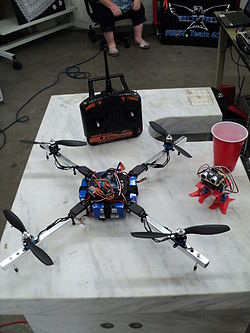
\includegraphics[width=0.3\textwidth]{./Pictures/250px-ReuseumMakerFaireQuadrotor.JPG}
    \caption{A Maker Faire quadcopter in Garden City, Idaho\cite{cite1}}\\
\end{figure}
\subsubsection{Flight Control}
\begin{figure}[h!]
  
  \centering
    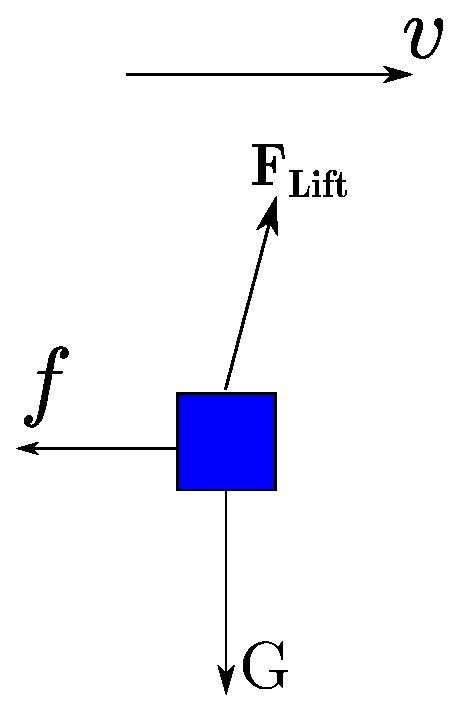
\includegraphics[width=0.3\textwidth]{./Pictures/flying.eps}
    \caption{The forces effected on the quadcopter while making stable movement.}\\
\end{figure}
%\newpage
\textbf{[ Hover ]}
\begin{figure}[H]
  
  \centering
    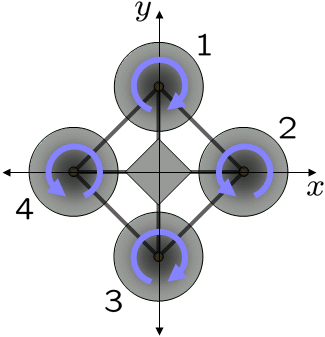
\includegraphics[width=0.3\textwidth]{./Pictures/Quadrotor_yaw_torque.png}
    \caption{The example model of quadcopter.}\\
\end{figure}


Each rotor porduces both thrust and torque. If all the rotors are spining at the same angular velocity, and as the example shows, with rotor 1,3 spining clockwise and rotor 2,4 spining counterclockwise, the angular acceleration on the yaw-axis will be zero. 
This is the method to hovering.

\textbf{[ Yaw ]}\\
\begin{figure}[H]
  
  \centering
    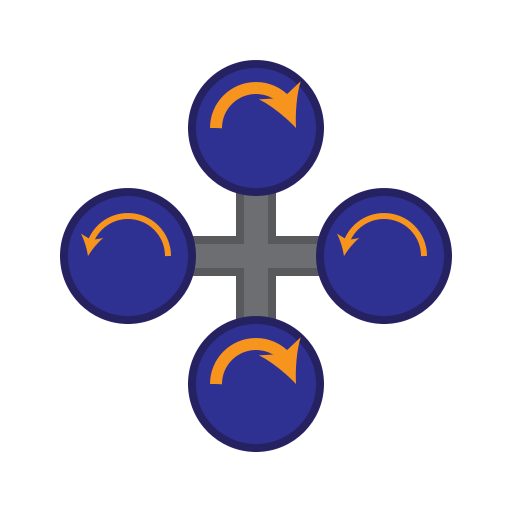
\includegraphics[width=0.3\textwidth]{./Pictures/yaw.png}
    \caption{Yaw control}
\end{figure}
The method of making yaw control can be done by adjusting the angular velocity of one pair of rotors.\\
\textbf{[ Pitch ]}\\
\begin{figure}[H]
  
  \centering
    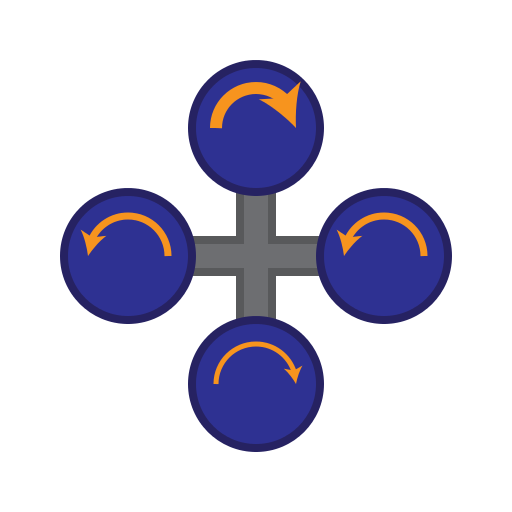
\includegraphics[width=0.3\textwidth]{./Pictures/pitch.png}
    \caption{Pitch control}
\end{figure}
The method of making pitch control can be done by increasing one rotor's spinning velocity and decreasing the opposite rotor's spinning velocity.\\
\textbf{[ Roll ]}\\
\begin{figure}[H]
  
  \centering
    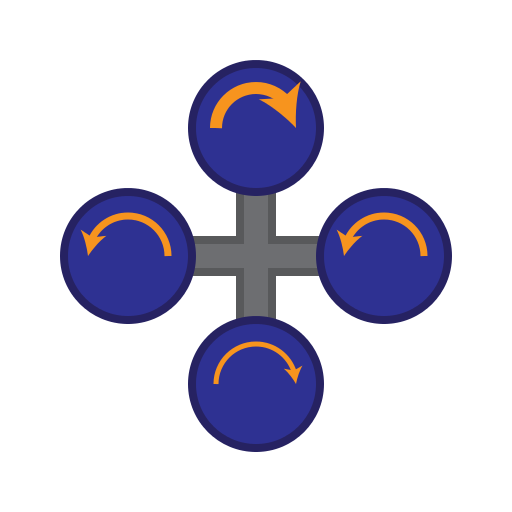
\includegraphics[width=0.3\textwidth, angle=90]{./Pictures/pitch.png}
    \caption{Roll control}
\end{figure}
The method of making roll control is similar to making pitch control.\\
It can be done by increasing one rotor's spinning velocity and decreasing the opposite rotor's spinning velocity.\\

\textbf{The eeeeeeeeeeasy way}\\
Use the ardupilot\cite{cite2} library.\\
\textbf{The harrrrrrrrrrd way}\\
Write the control system complete from scratch.\\
Which is possible, but might take a loooooooooong time.